\documentclass[a4paper]{article}

\def\npart {II}
\def\nterm {Michaelmas}
\def\nyear {2016}
\def\nlecturer {A. Ashton}
\def\ncourse {Integrable Systems}
\def\nlectures {TT.11}

% Imports
\ifx \nextra \undefined
  \usepackage[pdftex,
    hidelinks,
    pdfauthor={Dexter Chua},
    pdfsubject={Cambridge Maths Notes: Part \npart\ - \ncourse},
    pdftitle={Part \npart\ - \ncourse},
  pdfkeywords={Cambridge Mathematics Maths Math \npart\ \nterm\ \nyear\ \ncourse}]{hyperref}
  \title{Part \npart\ - \ncourse}
\else
  \usepackage[pdftex,
    hidelinks,
    pdfauthor={Dexter Chua},
    pdfsubject={Cambridge Maths Notes: Part \npart\ - \ncourse\ (\nextra)},
    pdftitle={Part \npart\ - \ncourse\ (\nextra)},
  pdfkeywords={Cambridge Mathematics Maths Math \npart\ \nterm\ \nyear\ \ncourse\ \nextra}]{hyperref}

  \title{Part \npart\ - \ncourse \\ {\Large \nextra}}
\fi

\author{Lectured by \nlecturer \\\small Notes taken by Dexter Chua}
\date{\nterm\ \nyear}

\usepackage{alltt}
\usepackage{amsfonts}
\usepackage{amsmath}
\usepackage{amssymb}
\usepackage{amsthm}
\usepackage{booktabs}
\usepackage{caption}
\usepackage{enumitem}
\usepackage{fancyhdr}
\usepackage{graphicx}
\usepackage{mathtools}
\usepackage{microtype}
\usepackage{multirow}
\usepackage{pdflscape}
\usepackage{pgfplots}
\usepackage{siunitx}
\usepackage{tabularx}
\usepackage{tikz}
\usepackage{tkz-euclide}
\usepackage[normalem]{ulem}
\usepackage[all]{xy}

\pgfplotsset{compat=1.12}

\pagestyle{fancyplain}
\lhead{\emph{\nouppercase{\leftmark}}}
\ifx \nextra \undefined
  \rhead{
    \ifnum\thepage=1
    \else
      \npart\ \ncourse
    \fi}
\else
  \rhead{
    \ifnum\thepage=1
    \else
      \npart\ \ncourse\ (\nextra)
    \fi}
\fi
\usetikzlibrary{arrows}
\usetikzlibrary{decorations.markings}
\usetikzlibrary{decorations.pathmorphing}
\usetikzlibrary{positioning}
\usetikzlibrary{fadings}
\usetikzlibrary{intersections}
\usetikzlibrary{cd}

\newcommand*{\Cdot}{\raisebox{-0.25ex}{\scalebox{1.5}{$\cdot$}}}
\newcommand {\pd}[2][ ]{
  \ifx #1 { }
    \frac{\partial}{\partial #2}
  \else
    \frac{\partial^{#1}}{\partial #2^{#1}}
  \fi
}

% Theorems
\theoremstyle{definition}
\newtheorem*{aim}{Aim}
\newtheorem*{axiom}{Axiom}
\newtheorem*{claim}{Claim}
\newtheorem*{cor}{Corollary}
\newtheorem*{defi}{Definition}
\newtheorem*{eg}{Example}
\newtheorem*{fact}{Fact}
\newtheorem*{law}{Law}
\newtheorem*{lemma}{Lemma}
\newtheorem*{notation}{Notation}
\newtheorem*{prop}{Proposition}
\newtheorem*{thm}{Theorem}

\renewcommand{\labelitemi}{--}
\renewcommand{\labelitemii}{$\circ$}
\renewcommand{\labelenumi}{(\roman{*})}

\let\stdsection\section
\renewcommand\section{\newpage\stdsection}

% Strike through
\def\st{\bgroup \ULdepth=-.55ex \ULset}

% Maths symbols
\newcommand{\bra}{\langle}
\newcommand{\ket}{\rangle}

\newcommand{\N}{\mathbb{N}}
\newcommand{\Z}{\mathbb{Z}}
\newcommand{\Q}{\mathbb{Q}}
\renewcommand{\H}{\mathbb{H}}
\newcommand{\R}{\mathbb{R}}
\newcommand{\C}{\mathbb{C}}
\newcommand{\Prob}{\mathbb{P}}
\renewcommand{\P}{\mathbb{P}}
\newcommand{\E}{\mathbb{E}}
\newcommand{\F}{\mathbb{F}}
\newcommand{\cU}{\mathcal{U}}
\newcommand{\RP}{\mathbb{RP}}
\newcommand{\CP}{\mathbb{CP}}

\newcommand{\ph}{\,\cdot\,}

\DeclareMathOperator{\sech}{sech}
\DeclareMathOperator{\cosech}{cosech}
\DeclareMathOperator{\cosec}{cosec}

\DeclareMathOperator{\covol}{covol}
\DeclareMathOperator{\vol}{vol}

\let\Im\relax
\let\Re\relax
\DeclareMathOperator{\Im}{Im}
\DeclareMathOperator{\Re}{Re}
\DeclareMathOperator{\im}{im}
\DeclareMathOperator{\image}{image}
\DeclareMathOperator{\Ann}{Ann}

\DeclareMathOperator*{\res}{res}
\DeclareMathOperator{\Res}{Res}
\DeclareMathOperator{\Ind}{Ind}

\DeclareMathOperator{\tr}{tr}
\DeclareMathOperator{\diag}{diag}
\DeclareMathOperator{\rank}{rank}
\DeclareMathOperator{\card}{card}
\DeclareMathOperator{\spn}{span}
\DeclareMathOperator{\adj}{adj}

\DeclareMathOperator{\erf}{erf}
\DeclareMathOperator{\erfc}{erfc}

\DeclareMathOperator{\ord}{ord}
\DeclareMathOperator{\Sym}{Sym}

\DeclareMathOperator{\sgn}{sgn}
\DeclareMathOperator{\orb}{orb}
\DeclareMathOperator{\stab}{stab}
\DeclareMathOperator{\ccl}{ccl}

\DeclareMathOperator{\lcm}{lcm}
\DeclareMathOperator{\hcf}{hcf}

\DeclareMathOperator{\Int}{Int}
\DeclareMathOperator{\id}{id}

\DeclareMathOperator{\betaD}{beta}
\DeclareMathOperator{\gammaD}{gamma}
\DeclareMathOperator{\Poisson}{Poisson}
\DeclareMathOperator{\binomial}{binomial}
\DeclareMathOperator{\multinomial}{multinomial}
\DeclareMathOperator{\Bernoulli}{Bernoulli}
\DeclareMathOperator{\like}{like}

\DeclareMathOperator{\var}{var}
\DeclareMathOperator{\cov}{cov}
\DeclareMathOperator{\bias}{bias}
\DeclareMathOperator{\mse}{mse}
\DeclareMathOperator{\corr}{corr}

\DeclareMathOperator{\otp}{otp}
\DeclareMathOperator{\dom}{dom}

\DeclareMathOperator{\Root}{Root}
\DeclareMathOperator{\supp}{supp}
\DeclareMathOperator{\rel}{rel}
\DeclareMathOperator{\Hom}{Hom}
\DeclareMathOperator{\Aut}{Aut}
\DeclareMathOperator{\Gal}{Gal}
\DeclareMathOperator{\Mat}{Mat}
\DeclareMathOperator{\End}{End}
\DeclareMathOperator{\Char}{char}
\DeclareMathOperator{\ev}{ev}
\DeclareMathOperator{\St}{St}
\DeclareMathOperator{\Lk}{Lk}
\DeclareMathOperator{\disc}{disc}
\DeclareMathOperator{\Isom}{Isom}
\DeclareMathOperator{\length}{length}
\DeclareMathOperator{\energy}{energy}
\DeclareMathOperator{\area}{area}
\DeclareMathOperator{\Syl}{Syl}
\DeclareMathOperator{\cl}{cl}
\DeclareMathOperator{\fix}{fix}

\newcommand{\GL}{\mathrm{GL}}
\newcommand{\SL}{\mathrm{SL}}
\newcommand{\PGL}{\mathrm{PGL}}
\newcommand{\PSL}{\mathrm{PSL}}
\newcommand{\PSU}{\mathrm{PSU}}
\newcommand{\Or}{\mathrm{O}}
\newcommand{\SO}{\mathrm{SO}}
\newcommand{\U}{\mathrm{U}}
\newcommand{\SU}{\mathrm{SU}}

\renewcommand{\d}{\mathrm{d}}
\newcommand{\D}{\mathrm{D}}

\tikzset{->/.style = {decoration={markings,
                                  mark=at position 1 with {\arrow[scale=2]{latex'}}},
                      postaction={decorate}}}
\tikzset{<-/.style = {decoration={markings,
                                  mark=at position 0 with {\arrowreversed[scale=2]{latex'}}},
                      postaction={decorate}}}
\tikzset{<->/.style = {decoration={markings,
                                   mark=at position 0 with {\arrowreversed[scale=2]{latex'}},
                                   mark=at position 1 with {\arrow[scale=2]{latex'}}},
                       postaction={decorate}}}
\tikzset{->-/.style = {decoration={markings,
                                   mark=at position #1 with {\arrow[scale=2]{latex'}}},
                       postaction={decorate}}}
\tikzset{-<-/.style = {decoration={markings,
                                   mark=at position #1 with {\arrowreversed[scale=2]{latex'}}},
                       postaction={decorate}}}

\tikzset{circ/.style = {fill, circle, inner sep = 0, minimum size = 3}}
\tikzset{mstate/.style={circle, draw, blue, text=black, minimum width=0.7cm}}

\definecolor{mblue}{rgb}{0.2, 0.3, 0.8}
\definecolor{morange}{rgb}{1, 0.5, 0}
\definecolor{mgreen}{rgb}{0.1, 0.4, 0.2}
\definecolor{mred}{rgb}{0.5, 0, 0}

\def\drawcirculararc(#1,#2)(#3,#4)(#5,#6){%
    \pgfmathsetmacro\cA{(#1*#1+#2*#2-#3*#3-#4*#4)/2}%
    \pgfmathsetmacro\cB{(#1*#1+#2*#2-#5*#5-#6*#6)/2}%
    \pgfmathsetmacro\cy{(\cB*(#1-#3)-\cA*(#1-#5))/%
                        ((#2-#6)*(#1-#3)-(#2-#4)*(#1-#5))}%
    \pgfmathsetmacro\cx{(\cA-\cy*(#2-#4))/(#1-#3)}%
    \pgfmathsetmacro\cr{sqrt((#1-\cx)*(#1-\cx)+(#2-\cy)*(#2-\cy))}%
    \pgfmathsetmacro\cA{atan2(#2-\cy,#1-\cx)}%
    \pgfmathsetmacro\cB{atan2(#6-\cy,#5-\cx)}%
    \pgfmathparse{\cB<\cA}%
    \ifnum\pgfmathresult=1
        \pgfmathsetmacro\cB{\cB+360}%
    \fi
    \draw (#1,#2) arc (\cA:\cB:\cr);%
}
\newcommand\getCoord[3]{\newdimen{#1}\newdimen{#2}\pgfextractx{#1}{\pgfpointanchor{#3}{center}}\pgfextracty{#2}{\pgfpointanchor{#3}{center}}}

\def\Xint#1{\mathchoice
   {\XXint\displaystyle\textstyle{#1}}%
   {\XXint\textstyle\scriptstyle{#1}}%
   {\XXint\scriptstyle\scriptscriptstyle{#1}}%
   {\XXint\scriptscriptstyle\scriptscriptstyle{#1}}%
   \!\int}
\def\XXint#1#2#3{{\setbox0=\hbox{$#1{#2#3}{\int}$}
     \vcenter{\hbox{$#2#3$}}\kern-.5\wd0}}
\def\ddashint{\Xint=}
\def\dashint{\Xint-}


\begin{document}
\maketitle
{\small
\noindent\emph{Part IB Methods, and Complex Methods or Complex Analysis are essential; Part II Classical Dynamics is desirable.}

\vspace{10pt}
\noindent Integrability of ordinary differential equations: Hamiltonian systems and the Arnol'd--Liouville Theorem (sketch of proof). Examples.\hspace*{\fill}[3]

\vspace{5pt}
\noindent Integrability of partial differential equations: The rich mathematical structure and the universality of the integrable nonlinear partial differential equations (Korteweg-de Vries, sine-Gordon). Backlund transformations and soliton solutions.\hspace*{\fill}[2]

\vspace{5pt}
\noindent The inverse scattering method: Lax pairs. The inverse scattering method for the KdV equation, and other integrable PDEs. Multi soliton solutions. Zero curvature representation. \hspace*{\fill}[6]

\vspace{5pt}
\noindent Hamiltonian formulation of soliton equations.\hspace*{\fill}[2]

\vspace{5pt}
\noindent Painleve equations and Lie symmetries: Symmetries of differential equations, the ODE reductions of certain integrable nonlinear PDEs, Painleve equations.\hspace*{\fill}[3]%
}

\tableofcontents
\setcounter{section}{-1}
\section{Introduction}
What is an integrable system? Unfortunately, an integrable system is a something mathematicians have not yet managed to define properly. Intuitively, an integrable system is a differential equation we can ``integrate up'' directly. While in theory, integrable systems should be very rare, it happens that in nature, a lot of systems happen to be integrable. By exploiting the fact that they are integrable, we can solve them much more easily.

\section{Integrability of ODE's}
\subsection{Vector fields and flow maps}
For a vector field $\mathbf{V}: \R^m \to \R^m$, consider a differential equation for $\mathbf{x}(t) \in \R^m$,
\[
  \dot{\mathbf{x}} = \mathbf{V}(\mathbf{x}),\quad \mathbf{x}(0) = \mathbf{x}_0.
\]
In this course, we will assume the vector field $\mathbf{V}$ is ``nice'', in the sense that the solutions always exist and are unique, and are infinitely differentiable.

It is convenient to write the solution as
\[
  \mathbf{x}(t) = g^t \mathbf{x}_0,
\]
where $g^t: \R^m \to \R^m$ is called the \emph{flow map}. This has some nice properties:
\begin{prop}\leavevmode
  \begin{enumerate}
    \item $g_0 = \id$
    \item $g^{t + s} = g^t g^s$
    \item $(g^{t})^{-1} = g^{-t}$
  \end{enumerate}
\end{prop}
The proofs are left for the first example sheet.

We say that $\mathbf{V}$ is the \emph{infinitesimal generator} of the flow $g^t$. This is because
\[
  \mathbf{x}(\varepsilon) = g^\varepsilon \mathbf{x}_0 = \mathbf{x}(0) + \varepsilon \dot{\mathbf{x}}(0) + o(\varepsilon) = \mathbf{x}_0 + \varepsilon \mathbf{V}(\mathbf{x}_0) + o(\varepsilon).
\]
For two vector fields $\mathbf{V}_1, \mathbf{V}_2: \R^m \to \R^m$ which generate flows $g_1^t$ and $g_2^s$, we define the third vector field, the commutator, by
\[
  [\mathbf{V}_1, \mathbf{V}_2] = \left(\mathbf{V}_1 \cdot \frac{\partial}{\partial \mathbf{x}}\right) \mathbf{V}_2 - \left(\mathbf{V}_2 \cdot \frac{\partial}{\partial \mathbf{x}}\right) \mathbf{V}_1,
\]
where we write
\[
  \frac{\partial}{\partial \mathbf{x}} = \left(\frac{\partial}{\partial x_1}, \cdots, \frac{\partial}{\partial x_n}\right)^T.
\]
More explicitly, the $i$th component
\[
  [\mathbf{V}_1, \mathbf{V}_2]_i = \sum_{j = 1}^m (\mathbf{v}_1)_j \frac{\partial}{\partial x_j} (\mathbf{v}_2)_i - (\mathbf{v}_2)_j \frac{\partial}{\partial x_j} (\mathbf{v}_1)_i
\]
This is a very important concept, because we have
\begin{prop}
  \[
    [\mathbf{V}_1, \mathbf{V}_2] = 0 \Leftrightarrow g_1^t g_2^s = g_2^s g_1^t.
  \]
\end{prop}
This will be shown in the first example sheet.

Thus, to figure out if two flows commute, it suffices to check if their infinitesimal generates commutative.
\subsection{Phase space and Poisson brackets}
In this section, we are interested in dynamical problems on a $2n$-dimensional \emph{phase space} $M$. Points on $M$ are described by coordinates
\[
  (\mathbf{q}, \mathbf{p}) = (q_1, \cdots, q_n, p_1, \cdots, p_n).
\]
We tend to think of the $q_i$ are ``generalized positions'' of particles, and the $p_n$ as the ``generalized momentum'' coordinates. We will often write
\[
  \mathbf{x} = (\mathbf{q}, \mathbf{p})^T.
\]
We introduce a $2n \times 2n$ anti-symmetric matrix
\[
  J =
  \begin{pmatrix}
    0 & I_n\\
    -I_n & 0
  \end{pmatrix}.
\]
We are now going to define a \emph{Poisson bracket}.

\begin{defi}[Poisson bracket]
  For any two functions $f, g: M \to \R$, we define the \emph{Poisson bracket} by
  \[
    \{f, g\} = \frac{\partial f}{\partial \mathbf{x}} J \frac{\partial g}{\partial \mathbf{x}} = \frac{\partial f}{\partial \mathbf{q}} \cdot \frac{\partial g}{\partial \mathbf{p}} - \frac{\partial f}{\partial \mathbf{p}} \cdot \frac{\partial g}{\partial \mathbf{q}}.
  \]
\end{defi}

This has some obvious and not-so-obvious properties:
\begin{prop}\leavevmode
  \begin{enumerate}
    \item This is linear in each argument.
    \item This is antisymmetric, ie. $\{f, g\} = - \{g, f\}$.
    \item Leibniz property: $\{f, gh\} = \{f, g\}h + \{f, h\} g$.
    \item Jacobi identity: $\{f, \{g, h\}\} + \{g, \{h, f\}\} + \{h, \{f, g\}\} = 0$.
    \item
      \[
        \{q_i, q_j\} = \{p_i, p_j\} = 0,\quad \{q_i, p_j\} = \delta_{ij}.
      \]
  \end{enumerate}
\end{prop}

\subsection{Hamiltonian dynamics}
We will be interested in problems on $M$ of the following form:
\begin{defi}[Hamilton's equation]
  \emph{Hamilton's equation} is an equation of the form
  \[
    \dot{\mathbf{q}} = \frac{\partial H}{\partial \mathbf{p}},\quad \dot{\mathbf{p}} = -\frac{\partial H}{\partial \mathbf{q}}\tag{$*$}
  \]
  For some function $H: M \to \R$ called the \emph{Hamiltonian}.
\end{defi}
Just as we think of $\mathbf{q}$ and $\mathbf{p}$ as generalized position and momentum, we tend to think of $H$ as generalized energy.

Note that $(*)$ can be written as
\[
  \dot{\mathbf{x}} = J \frac{\partial H}{\partial \mathbf{x}}.
\]
Compare this to the equation
\[
  \dot{\mathbf{x}} = \mathbf{V}(\mathbf{x}), \quad \mathbf{x}(0) = \mathbf{x}_0.
\]
Assuming that $\mathbf{x}$ evolves according to Hamilton's equations, if $f: M \to \R$ is a smooth function, then by the chain rule, we have
\begin{align*}
  \frac{\d f}{\d t} &= \frac{\d}{\d t} f(\mathbf{q}(t), \mathbf{p}(t))\\
  &= \frac{\partial f}{\partial \mathbf{q}} \cdot \dot{\mathbf{q}} + \frac{\partial f}{\partial \mathbf{p}} \cdot \dot{\mathbf{p}}\\
  &= \frac{\partial f}{\partial \mathbf{q}} \cdot \frac{\partial H}{\partial \mathbf{p}} - \frac{\partial f}{\partial \mathbf{p}} \cdot \frac{\partial H}{\partial \mathbf{q}} \\
  &= \{f, H\}.
\end{align*}
In particular, we have
\[
  \frac{\d H}{\d t} = \{H, H\} = 0.
\]
So the Hamiltonian is constant!
\begin{eg}
  Consider a particle (of unit mass) with position $\mathbf{q} = (q_1, q_2, q_3)$ (in Cartesian coordinates) moving under the influence of a potential $U(\mathbf{q})$. By Newton's second law, we have
  \[
    \ddot{\mathbf{q}} = -\frac{\partial U}{\partial \mathbf{q}}.
  \]
  This is actually a Hamiltonian system. We define the momentum variables by
  \[
    p_i = \dot{q}_i,
  \]
  then we have
  \[
    \dot{\mathbf{x}} =
    \begin{pmatrix}
      \dot{\mathbf{q}}
      \dot{\mathbf{p}}
    \end{pmatrix}
    =
    \begin{pmatrix}
      \mathbf{p}\\
      -\frac{\partial U}{\partial \mathbf{q}}
    \end{pmatrix}
    = J \frac{\partial H}{\partial \mathbf{x}},
  \]
  with
  \[
    H = \frac{1}{2} \abs{\mathbf{p}}^2 + U(\mathbf{q}).
  \]
  This is just the usual energy! Indeed, we have
  \[
    \frac{\partial H}{\partial \mathbf{p}} = \mathbf{p},\quad \frac{\partial H}{\partial \mathbf{q}} = \frac{\partial H}{\partial \mathbf{q}}.
  \]
\end{eg}

\begin{defi}[Hamiltonian vector field]\index{Hamiltonian vector field}
  Given a Hamiltonian function $H$, the \emph{Hamiltonian vector field} is given by
  \[
    \mathbf{V}_H = J \frac{\partial H}{\partial \mathbf{x}}.
  \]
\end{defi}

We then see that the Hamiltonian vector field generates the Hamiltonian flow. More generally, for any $f: M \to \R$, we call
\[
  \mathbf{V}_f = J \frac{\partial f}{\partial \mathbf{x}}.
\]
This is the Hamiltonian vector field with respect to $f$ and $g$.

\begin{prop}
  We have
  \[
    [V_\mathbf{f}, V_\mathbf{g}] = - \mathbf{V}_{\{f, g\}}.
  \]
\end{prop}

\begin{proof}
  See first example sheet. % Fill in
\end{proof}

\begin{defi}[First integral]\index{first integral}
  Given a phase space $M$ with a Hamiltonian $H$, we call $f: M \to \R$ a \emph{first integral} of the Hamiltonian system if
  \[
    \{f, H\} = 0.
  \]
\end{defi}
The reason for the term ``first integral'' is historical --- when we solve a differential equation, we integrate the equation. Every time we integrate it, we obtain a new constant. And the first constant we obtain when we integrate is known as the first integral. However, for our purposes, we can just as well think of it as a constant of motion.

\begin{eg}
  Consider the two-body problem --- the Sun is fixed at the origin, and a planet has Cartesian coordinates $\mathbf{q} = (q_1, q_2, q_3)$. The equation of motion will be
  \[
    \ddot{\mathbf{q}} = - \frac{\mathbf{q}}{|\mathbf{q}|^3}.
  \]
  This is equivalent to the Hamiltonian system $\mathbf{p} = \dot{\mathbf{q}}$, with
  \[
    H = \frac{1}{2} |\mathbf{p}|^2 - \frac{1}{|\mathbf{q}|}.
  \]
  We have an angular momentum given by
  \[
    \mathbf{L} = \mathbf{q} \wedge \mathbf{p}.
  \]
  Working with coordinates, we have
  \[
    L_i = \varepsilon_{ijk} q_j p_k.
  \]
  We then have
  \begin{align*}
    \{L_i, H\} &= \frac{\partial L_i}{\partial q_\ell}\frac{\partial H}{\partial p_\ell} - \frac{\partial L_i}{\partial p_\ell} \frac{\partial H}{\partial q_\ell}\\
    &= \varepsilon_{ijk} \left(p_k \delta_{\ell j}p_\ell + \frac{q_j q_k}{|\mathbf{q}|^3}\right)\\
    &= \varepsilon_{ijk} \left(p_k p_j + \frac{q_j q_k}{|\mathbf{q}|^3}\right)\\
    &= 0,
  \end{align*}
  where we know the thing vanishes because we contracted a symmetric tensor with an antisymmetric one. So this is a first integral.

  Less interestingly, we know $H$ is also a first integral. In general, some Hamiltonian have many many first integrals.
\end{eg}

\begin{defi}[Involution]\index{involution}
  We say that two first integrals $F, G$ are in \emph{involution} if $\{F, G\} = 0$ (so $F$ and $G$ ``\emph{Poisson commute}'').
\end{defi}

\begin{defi}[Independent first integrals]\index{independent first integrals}
  A collection of functions $f_i: M \to \R$ are independent if at each $\mathbf{x} \in M$, the vectors $\frac{\partial f_i}{\partial \mathbf{x}}$ for $i = 1, \cdots, n$ are independent.
\end{defi}

\begin{defi}[Integrable system]\index{integrable system}
  A $2n$-dimensional Hamiltonian system $(M, H)$ is \emph{integrable} if there exists $n$ first integrals $\{f_i\}_{i = 1}^n$ that are independent and in involution (ie. $\{f_i, f_j\} = 0$ for all $i, j$).
\end{defi}
The word independent is very important, or else people will cheat, eg. take $H, 2H, e^H, H^2, \cdots$.

\begin{cor}
  Two-dimensional Hamiltonian systems are always integrable.
\end{cor}

We are now ready for the main section.
%\section{Action-angle coordinates and the Arnold-Liouville theorem}
\section{The Arnold-Liouville theorem}
Consider the Hamiltonian system
\[
  \dot{\mathbf{q}} = \frac{\partial H}{\partial \mathbf{q}},\quad \mathbf{p} = -\frac{\partial H}{\partial \mathbf{q}}.
\]
We do not expect a general coordinate change $(\mathbf{q}, \mathbf{p}) \mapsto (\mathbf{Q}(\mathbf{q}, \mathbf{q}), \mathbf{P}(\mathbf{q}, \mathbf{p}))$ to hold the form of Hamilton's equations, ie. we will no longer have
\[
  \dot{\mathbf{Q}} = \frac{\partial \tilde{H}}{\partial \mathbf{P}},\quad \dot{\mathbf{P}} = -\frac{\partial \tilde{H}}{\partial \mathbf{Q}},
\]
where $\tilde{H}(\mathbf{Q}, \mathbf{P}) = H(\mathbf{q}, \mathbf{p})$.

If we write $\mathbf{x} = (\mathbf{q}, \mathbf{p})$ and $\mathbf{y} = (\mathbf{Q}, \mathbf{P})$, then this is equivalent to asking if
\[
  \dot{\mathbf{x}} = J \frac{\partial H}{\partial \mathbf{x}} \quad\Rightarrow\quad \dot{\mathbf{y}} = J \frac{\partial \tilde{H}}{ \partial \mathbf{y}}.
\]
For example, if we just swap $\mathbf{p}$ and $\mathbf{q}$ around, the form of the equation changes (namely the signs go in the wrong place).

\begin{defi}[Canonical transformation]\index{canonical transformation}
  A coordinate change $(\mathbf{q}, \mathbf{p}) \mapsto (\mathbf{Q}, \mathbf{P})$ is called \emph{canonical} if it leaves Hamilton's equations invariant, ie. we have
  \[
    \dot{\mathbf{Q}} = \frac{\partial \tilde{H}}{\partial \mathbf{P}},\quad \dot{\mathbf{P}} = -\frac{\partial \tilde{H}}{\partial \mathbf{Q}},
  \]
\end{defi}

\begin{eg}
  The simplest possible case of a canonical transformation is a linear transformation. Consider a linear change of coordinates given by
  \[
    \mathbf{x} \mapsto \mathbf{y}(\mathbf{x}) = A\mathbf{x}.
  \]
  We claim that this is canonical iff $AJA^t = J$, ie. that $A$ is \term{symplectic}.

  Indeed, by linearity, we have
  \[
    \dot{\mathbf{y}} = A\dot{\mathbf{x}} = AJ\frac{\partial H}{\mathbf{x}}.
  \]
  Setting $\tilde{\mathbf{H}}(\mathbf{y} = H(\mathbf{x})$, we have
  \[
    \frac{\partial H}{\partial x_i} = \frac{\partial y_j}{\partial x_i} \frac{\partial \tilde{H}(\mathbf{y})}{\partial y_j} = A_{ji} \frac{\partial \tilde{H}(\mathbf{y})}{\partial y_j}(\mathbf{y}) = \left[A^T \frac{\partial \tilde{H}}{\partial \mathbf{y}}\right]_i.
  \]
  Putting this back in, we have
  \[
    \dot{\mathbf{y}} = AJA^T \frac{\partial\tilde{H}}{\partial \mathbf{y}}.
  \]
  So $\mathbf{y} \mapsto \mathbf{y}(\mathbf{x})$ is canonical if $J = AJA^T$.
\end{eg}

What about more general cases? Recall from IB Analysis II that a map is differentiable if it is ``locally linear''. Now Hamilton's equations are purely local equations, so we might expect the following:
\begin{prop}
  A map $\mathbf{x} \mapsto \mathbf{y}(\mathbf{x})$ is canonical iff $D\mathbf{y}$ is symplectic, ie.
  \[
    D\mathbf{y} J (D\mathbf{y})^T = J.
  \]
\end{prop}

Now could we find a canonical transformation $(\mathbf{q}, \mathbf{p}) \mapsto (\mathbf{Q}, \mathbf{P})$ such that $\tilde{H}$ depends only on $\mathbf{P}$. If this happened, then Hamilton's equations reduce to
\[
  \dot{\mathbf{Q}} = \frac{\partial \tilde{H}}{\partial \mathbf{P}}(\mathbf{P}),\quad \dot{\mathbf{P}} = -\frac{\partial \tilde{H}}{\partial \mathbf{Q}} = 0.
\]
So $\mathbf{P}(t) = \mathbf{P}_0$ is a constant. Since the right hand side of the first equation depends only on $\mathbf{P}$, we find that $\dot{\mathbf{Q}}$ is also constant! So $\mathbf{Q} = \mathbf{Q}_0 + \Omega t$, where
\[
  \Omega = \frac{\partial \tilde{H}}{\partial \mathbf{P}} (\mathbf{P}_0).
\]
So if we could find a good canonical transformation, the solution falls out easily! It turns out that if a system is integrable, then we can indeed find such coordinates.

We are now going to prove the Arnold-Liouville theorem. Before we do that in full generality, we first do it in a specific case, and see how the proof actually works out.

\begin{eg}
  Consider the harmonic oscillator with Hamiltonian
  \[
    H(q, p) = \frac{1}{2}p^2 + \frac{1}{2}\omega^2 q^2.
  \]
  Since is a 2-dimensional system, so we only need a single first integral. Since $H$ is a first integral for trivial reasons, this is an integrable Hamiltonian system.

  We can actually draw the lines on which $H$ is constant --- they are just ellipses:
  \begin{center}
    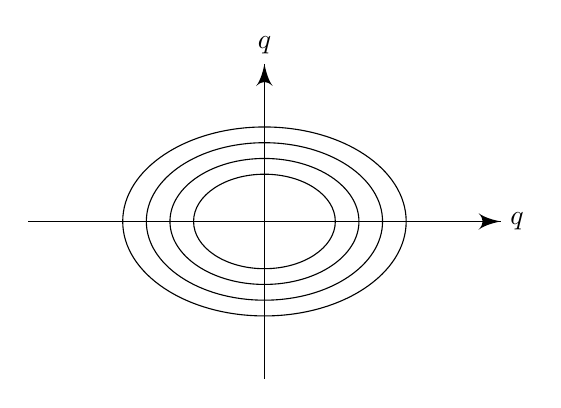
\begin{tikzpicture}
      \draw [->] (-3, 0) -- (3, 0) node [right] {$q$};
      \draw [->] (0, -2) -- (0, 2) node [above] {$q$};

      \foreach \x in {0.6, 0.8, 1, 1.2} {
        \begin{scope}[scale=\x]
          \draw ellipse (1.5 and 1);
        \end{scope}
      }
    \end{tikzpicture}
  \end{center}
  We note that the ellipses are homeomorphic to $S^1$. Now we introduce the coordinate transformation $(q, p) \mapsto (\phi, I)$, defined by
  \[
    q = \sqrt{\frac{2I}{\omega}} \sin \phi,\quad p = \sqrt{2I\omega} \cos \phi,
  \]
  For the purpose of this example, we can suppose we obtained this formula through divine inspiration. However, in the Arnold-Liouville theorem, we will provide a general way of coming up with these formulas.

  We can manually show that this transformation is canonical (it is actually easier to show that the inverse map $(\phi, I) \mapsto (q, p)$ is canonical). We also have that
  \[
    \tilde{H}(\phi, I) = H(q(\phi, I), p(\phi, I)) = \omega I.
  \]
  This is really nice. There is no $\phi$! Now Hamilton's equations become
  \[
    \dot\phi = \frac{\partial \tilde{H}}{ \partial I} = \omega,\quad \dot{I} = -\frac{\partial \tilde{H}}{\partial \phi} = 0.
  \]
  We can integrate up to obtain
  \[
    \phi(t) = \phi_0 + \omega t,\quad I(t) = I_0.
  \]
  It is fun to consider the integral along paths of constant $H$:
  \begin{align*}
    \frac{1}{2\pi}\oint p \;\d q &= \frac{1}{2\pi} \int_0^{2\pi}p(\phi, I) \left(\frac{\partial q}{\partial \phi} \;\d \phi + \frac{\partial q}{\partial I} \;\d I\right)\\
    &= \frac{1}{2\pi} \int_0^{2\pi}p(\phi, I) \left(\frac{\partial q}{\partial \phi} \;\d \phi\right)\\
    &= \frac{1}{2\pi} \int_0^{2\pi} \sqrt{\frac{2I}{\omega}}\sqrt{2I\omega} \cos^2 \phi \;\d \phi\\
    &= I
  \end{align*}
  This is interesting. We didn't know how we obtained $I$, but in fact we can obtain it by performing an integral like this.
\end{eg}
There are two things to take away from this.
\begin{enumerate}
  \item The motion takes place in $S^1$
  \item We got $I$ by performing $\frac{1}{2\pi}\oint p \;\d q$.
\end{enumerate}
These two ideas are essentially what we are going to prove for general Hamiltonian system.

% insert something about generating functions

\begin{thm}[Arnold-Liouville theorem]\index{Arnold-Liouville theorem}
  We let $(M, H)$ be an integrable $2n$-dimensional Hamiltonian system with independent, involutive first integrals $f_1, \cdots, f_n$, where $f_1 = H$. For any fixed $\mathbf{c} \in \R^n$, we set
  \[
    M_\mathbf{c} = \{(\mathbf{q}, \mathbf{p}) \in M: f_i(\mathbf{q}, \mathbf{p}) = c_i, i =1 , \cdots, n\}.
  \]
  Then
  \begin{enumerate}
    \item $M_\mathbf{c}$ is a smooth $n$-dimensional surface in $M$. If $M_\mathbf{c}$ is compact and connected, then it is diffeomorphic to
      \[
        T^n = S^1 \times \cdots \times S^1.
      \]
    \item (\ldots) % fill in
  \end{enumerate}
\end{thm}

\begin{proof}[Proof sketch]
  We first show that $M_\mathbf{c}$ is smooth and $n$-dimensional. We will handwave through this part. The proper proof follows easily from techniques found in IID Differential geometry using the implicit function theorem. We know $M_\mathbf{c}$ is a surface defined by $n$ constraints, while the whole phase space $M$ has $2n$ degrees of freedom. So the remaining number of degrees of freedom on $M_\mathbf{c}$ is $n$. The key that makes this work is that the constraints are independent, which is the condition that allows us to apply the implicit function theorem.

  We now show that $M_\mathbf{c}$ is diffeomorphic to the torus if it is compact and connected. Consider the Hamiltonian vector fields defined by
  \[
    \mathbf{V}_{f_i} = J \frac{\partial f_i}{\partial \mathbf{x}}.
  \]
  We claim that these are \emph{tangent} to the surface $M_\mathbf{c}$. Indeed, we want to see if any of the $\{f_j\}$ change in the direction of $\mathbf{V}_{f_i}$. We can compute
  \[
    \left(\mathbf{V}_{f_i} \cdot \frac{\partial}{\partial \mathbf{x}}\right)f_j = \frac{\partial f_j}{\partial \mathbf{x}} J \frac{\partial f_i}{\partial \mathbf{x}} = \{f_j, f_i\} = 0.
  \]
  Since this vanishes, we know that $\mathbf{V}_{f_i}$ is a tangent a tangent to the surface. So the flow maps $\{g_i\}$ map $M_\mathbf{c}$ to itself. Also, we know that the flow maps commute. Indeed, we can compute
  \[
    [\mathbf{V}_{f_i}, \mathbf{V}_{f_j}] = -\mathbf{V}_{\{f_i, f_j\}} = -\mathbf{V}_{0} = 0.
  \]
  So we have a whole bunch of commuting flow maps from $M_\mathbf{c}$ to itself. We set
  \[
    g^\mathbf{t} = g_1^{t_1} g_2^{t_2} \cdots g_n^{t_n},
  \]
  where $\mathbf{t} \in \R^n$. Then because of commutativity, we have
  \[
    g^{\mathbf{t}_1 + \mathbf{t}_2} = g^{\mathbf{t}_1}g^{\mathbf{t}_2}.
  \]
  So this is gives a group action of $\R^n$ on the surface $M_\mathbf{c}$. We fix $\mathbf{x} \in M_\mathbf{c}$. We define
  \[
    \stab(\mathbf{x}) = \{\mathbf{t} \in \R^n: g^\mathbf{t}\mathbf{x} = \mathbf{x}\}.
  \]
  We introduce the map
  \[
    \phi: \frac{\R^n}{\stab(\mathbf{x})} \to M_\mathbf{c}
  \]
  given by $\phi(\mathbf{t}) = g^{\mathbf{t}}\mathbf{x}$. By the orbit-stabilizer theorem, this gives a bijection between $\R^n/\stab(\mathbf{x})$ and the orbit of $\mathbf{x}$. It can be shown that the orbit of $\mathbf{x}$ is exactly the connected component of $\mathbf{x}$. Now if $M_\mathbf{c}$ is connected, then this must be the whole of $\mathbf{x}$! By general differential geometry theory, we get that this map is indeed a diffeomorphism.

  We know that $\stab(\mathbf{x})$ is a subgroup of $\R^n$, and if the $g_i$ are non-trivial, it can be seen (at least intuitively) that this is discrete. Thus, it must be isomorphic to something of the form $\Z^k$ with $1 \leq k \leq n$.

  So we have
  \[
    M_\mathbf{c} \cong \R^n / \stab(\mathbf{x}) \cong \R^n/\Z^k \cong \cong \R^k/\Z^k \times \R^{n - k} \cong T^k \times \R^{n - k}.
  \]
  Now if $M_\mathbf{c}$ is compact, we must have $n - k = 0$, ie. $n = k$, so that we have no factors of $\R$. So $M_\mathbf{c} \cong T^n$.

  We are now done with the topological part. We are now going to construct the action-angle coordinates concretely.

  For simplicity of presentation, we only do it in the case when $n = 2$. The proof for higher dimensions is entirely analogous, except that we need to use a higher-dimensional analogue of Green's theorem, which we do not currently have.

  We note that it is currently trivial to re-parameterize the phase space with coordinates $(\mathbf{Q}, \mathbf{P})$ such that $\mathbf{P}$ is constant within the Hamiltonian flow, and each coordinate of $\mathbf{Q}$ takes values in $S^1$. Indeed, we just put $\mathbf{P} = \mathbf{c}$ and use the diffeomorphism $T^n \cong M_\mathbf{c}$ to parameterize each $M_\mathbf{c}$ as a product of $n$ copies of $S^n$. However, this is not good enough, because such an arbitrary transformation will almost certainly not be canonical. So we shall try to find a more natural and in fact canonical way of parametrizing our phase space.

  We first work on the generalized momentum part. We want to replace $\mathbf{c}$ with something nicer. We will do something analogous to the simple harmonic oscillator we've got.

  So we fix a $\mathbf{c}$, and try to come up with some numbers $\mathbf{I}$ that labels this $M_\mathbf{c}$. Recall that our surface $M_\mathbf{c}$ looks like a torus:
  \begin{center}
    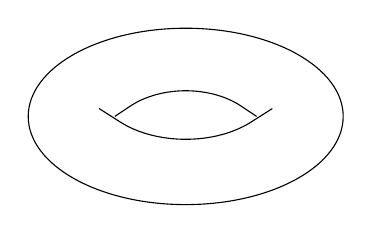
\begin{tikzpicture}
      \draw (0,0) ellipse (2 and 1.12);
      \path[rounded corners=24pt] (-.9,0)--(0,.6)--(.9,0) (-.9,0)--(0,-.56)--(.9,0);
      \draw[rounded corners=28pt] (-1.1,.1)--(0,-.6)--(1.1,.1);
      \draw[rounded corners=24pt] (-.9,0)--(0,.6)--(.9,0);
    \end{tikzpicture}
  \end{center}
  Up to continuous deformation of loops, we see that there are two non-trivial ``single'' loops in the torus, given by the red and blue loops:
  \begin{center}
    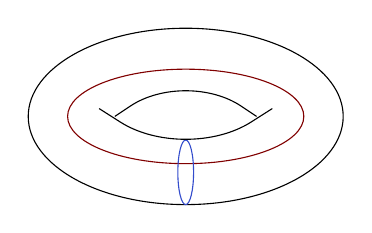
\begin{tikzpicture}
      \draw (0,0) ellipse (2 and 1.12);
      \draw [mred] (0,0) ellipse (1.5 and 0.6);

      \draw [mblue] (0, -0.71) ellipse (0.1 and 0.41);
      \path [rounded corners=24pt] (-.9,0)--(0,.6)--(.9,0) (-.9,0)--(0,-.56)--(.9,0);
      \draw [rounded corners=28pt] (-1.1,.1)--(0,-.6)--(1.1,.1);
      \draw [rounded corners=24pt] (-.9,0)--(0,.6)--(.9,0);
    \end{tikzpicture}
  \end{center}
  More generally, for an $n$ torus, we have $n$ such distinct loops $\Gamma_1, \cdots, \Gamma_n$. More concretely, after identifying $M_\mathbf{c}$ with $S^n$, these are the loops given by
  \[
    \{0\} \times \cdots \times \{0\} \times S^1 \times \{0\} \times \cdots \times \{0\} \subseteq S^1.
  \]
  We now attempt to define:
  \[
    I_j = \frac{1}{2\pi} \oint_{\Gamma_j} \mathbf{p}\cdot \d \mathbf{q},
  \]
  This is just like the formula we had for the simple harmonic oscillator.% Homologically, these are given by generators of the $1$-cycles in $H_1((M_\mathbf{c})$.

  We want to make sure this is well-defined --- recall that $\Gamma_i$ actually represents a \emph{class} of loops identified under continuous deformation. What if we picked a different loop?

  % insert picture.

  On $M_\mathbf{c}$, we have the equation
  \[
    f_i(\mathbf{q}, \mathbf{p}) = \mathbf{c}_i.
  \]
  We assume that we can invert this equation for $\mathbf{p}$ locally, ie. write
  \[
    \mathbf{p} = \mathbf{p}(\mathbf{q}, \mathbf{c}).
  \]
  The condition for being able to do so is just
  \[
    \det\left(\frac{\partial f_i}{\partial p_j}\right) \not= 0,
  \]
  which is not hard.

  Then by definition, the following holds identically:
  \[
    f_i(\mathbf{q}, \mathbf{p}(\mathbf{q}, \mathbf{c})) = c_i.
  \]
  We an then differentiate this with respect to $q_k$ to obtain
  \[
    \frac{\partial f_i}{\partial q_k} + \frac{\partial f_i}{\partial p_\ell} \frac{\partial p_\ell}{\partial q_k} = 0
  \]
  on $M_\mathbf{c}$. Now recall that the $\{f_i\}$'s are in involution. So on $M_\mathbf{c}$, we have
  \begin{align*}
    0 &= \{f_i, f_j\} \\
    &= \frac{\partial f_i}{\partial q_k} \frac{\partial f_j}{\partial p_k} - \frac{\partial f_i}{\partial p_k} \frac{\partial f_j}{\partial q_k}\\
    &= \left(-\frac{\partial f_i}{\partial p_\ell} \frac{\partial p_\ell}{\partial q_k}\right)\frac{\partial f_j}{\partial p_k} - \frac{\partial f_i}{\partial p_k}\left(-\frac{\partial f_j}{\partial p_\ell} \frac{\partial p_\ell}{\partial q_k}\right)\\
    &= \left(-\frac{\partial f_i}{\partial p_k} \frac{\partial p_k}{\partial q_\ell}\right)\frac{\partial f_j}{\partial p_\ell} - \frac{\partial f_i}{\partial p_k}\left(-\frac{\partial f_j}{\partial p_\ell} \frac{\partial p_\ell}{\partial q_k}\right)\\
    &= \frac{\partial f_i}{\partial p_k} \left(\frac{\partial p_\ell}{\partial q_k} - \frac{\partial p_k}{\partial q_\ell}\right) \frac{\partial f_j}{\partial p_\ell}.
  \end{align*}
  Recall that the determinants of the matrices $\frac{\partial f_i}{\partial p_k}$ and $\frac{\partial f_j}{\partial p_\ell}$ are non-zero. So the middle matrix must vanish! So we have
  \[
    \frac{\partial p_\ell}{\partial q_k} - \frac{\partial p_k}{\partial q_\ell} = 0.
  \]
  Since $\ell, k$ can only be $1, 2$ in this case, the only non-trivial thing this says is
  \[
    \frac{\partial p_1}{\partial q_2} - \frac{\partial p_2}{\partial q_1} = 0.
  \]
  Now suppose we have two loops $\Gamma_2$ and $\Gamma_2'$.
  % insert picture of \Gamma_2 and \Gamma_2' and surface A between them.
  Then we have
  \begin{align*}
    \left(\oint_{\Gamma_2} - \oint_{\gamma_2'}\right) \mathbf{p}\cdot \d \mathbf{q} &= \oint_{\partial A}\mathbf{p}\cdot \d \mathbf{q}\\
    &= \iint_A \left(\frac{\partial p_2}{\partial q_1} - \frac{\partial p_1}{\partial q_2}\right) \;\d q_1\;\d q_2\\
    &= 0
  \end{align*}
  by Green's theorem.

  So $I_j$ is well-defined, and
  \[
    \mathbf{I} = \mathbf{I}(\mathbf{c})
  \]
  is just a function of $c$.

  We will assume that we can invert this, so
  \[
    \mathbf{c} = \mathbf{c}(\mathbf{I}).
  \]
  We are now going to parametrize each $M_\mathbf{c}$. We are going to do so via generating functions.

  We arbitrarily pick a point $\mathbf{x}_0$, and define the generating function
  \[
    S(\mathbf{q}, \mathbf{I}) = \int_{\mathbf{x}_0}^\mathbf{x} \mathbf{p}(\mathbf{q}', \mathbf{c}(\mathbf{I})) \cdot \d \mathbf{q}',
  \]
  where $\mathbf{x} = (\mathbf{q}, \mathbf{p})$. This is just a function of $\mathbf{q}$ (and thus $\mathbf{x}$), and $\mathbf{I}$. However, this is not well-defined, because we haven't said how we are going to integrate from $\mathbf{x}_0$ to $\mathbf{x}$. We are going to pick paths arbitrarily, but we want to make sure it is well-defined. Suppose we change from a path $\gamma_1$ to $\gamma_2$ by a little bit, and they enclose a boundary $B$.

  % insert picture

  Then we have
  \[
    S(\mathbf{q}, \mathbf{I}) \mapsto S(\mathbf{q}, \mathbf{I}) + \oint_{\partial B} \mathbf{p} \cdot \d \mathbf{q}.
  \]
  Again, we are integrating $\mathbf{p} \cdot \d\mathbf{q}$ around a boundary, so there is no change.

  But what if we do something crazy, like

  % insert picture

  Then what we have effectively got is that we added a loop $\Gamma_2$ to our path, and this contributes a factor of $2\pi I_j$. So we have
  \[
    S(\mathbf{q}, \mathbf{I}) \mapsto S(\mathbf{q}, I) + 2\pi I_j.
  \]
  This is the only thing that can happen. So differentiating with repsect to $I$, we know that
  \[
    \frac{\partial S}{\partial \mathbf{I}}
  \]
  is well-defined modulo $2\pi$. These are the \emph{angles}
  \[
    \boldsymbol\phi = \frac{\partial S}{\partial \mathbf{I}}.
  \]
  Now also note that
  \[
    \frac{\partial S}{\partial \mathbf{q}} = \mathbf{p}.
  \]
  Indeed, we can write
  \[
    S = \int_{\mathbf{x}_0}^\mathbf{x} \mathbf{F} \cdot \d \mathbf{x}',
  \]
  where
  \[
    \mathbf{F} = (\mathbf{p}, 0).
  \]
  So we have
  \[
    \frac{\partial S}{\partial \mathbf{x}} = \mathbf{F},
  \]
  so
  \[
    \frac{\partial S}{\partial \mathbf{q}} = \mathbf{p}.
  \]
  In summary, we have constructed on $M_\mathbf{c}$ the following: $\mathbf{I}= \mathbf{I}(\mathbf{c})$, $S(\mathbf{q}, I)$, and
  \[
    \boldsymbol\phi = \frac{\partial S}{\partial \mathbf{I}},\quad \mathbf{p} = \frac{\partial S}{\partial \mathbf{q}}.
  \]
  So $S$ is a generator for the canonical transformation, and $(\mathbf{q}, \mathbf{p}) \mapsto (\boldsymbol\phi, \mathbf{I})$ is a canonical transformation.

  Note that at any point $\mathbf{x}$, we know $\mathbf{c} = \mathbf{f}(\mathbf{x})$. So $I(\mathbf{c}) = I(\mathbf{f})$ depends on the first integrals only. So we have
  \[
    \dot{\mathbf{I}} = 0.
  \]
  So Hamilton's equations become
  \[
    \dot{\boldsymbol\phi} = \frac{\partial \tilde{H}}{\partial \mathbf{I}},\quad \dot{\mathbf{I}} = 0 = \frac{\partial \tilde{H}}{\partial \boldsymbol\phi}.
  \]
  So the new Hamiltonian depends only on $\mathbf{I}$. So we can integrate up and get
  \[
    \boldsymbol\phi(t) = \boldsymbol\phi_0 + \Omega t,\quad \mathbf{I}(t) = I_0,
  \]
  where
  \[
    \Omega = \frac{\partial\tilde{H}}{\partial I}(I_0).
  \]
\end{proof}
To summarize, to integrate up an integrable Hamiltonian system, we identify the different cycles $\Gamma_1, \cdots, \Gamma_n$ on $M_\mathbf{c}$. We then construct
\[
  I_j = \frac{1}{2\pi} \oint_{\Gamma_j} \mathbf{p}\cdot \d \mathbf{q},
\]
where $\mathbf{p} = \mathbf{p}(\mathbf{q}, \mathbf{c})$. We then invert this to say
\[
  \mathbf{c} = \mathbf{c}(\mathbf{I}).
\]
We then compute
\[
  \boldsymbol\phi = \frac{\partial S}{\partial I_j},
\]
where
\[
  S = \int_{\mathbf{x}_0}^{\mathbf{x}} \mathbf{p}(\mathbf{q}', \mathbf{c}(\mathbf{I})) \cdot \d \mathbf{q}'.
\]
Now we do this with the Harmonic oscillator.
\begin{eg}
  In the harmonic oscillator, we have
  \[
    H(q, p) = \frac{1}{2}p^2 + \frac{1}{2}\omega^2 q^2.
  \]
  We then have
  \[
    M_\mathbf{c} = \left\{(q, p): \frac{1}{2} p^2 + \frac{1}{2}\omega^2 q^2 = c\right\}.
  \]
  The first part of the Arnold-Liouville theorem says this is diffeomorphic to $T^1 = S^1$, which it is! The next step is to pick a loop, and there is an obvious one --- the circle itself. We write
  \[
    p = p(q, c) = \pm \sqrt{2c - \omega^2 q^2}
  \]
  on $M_\mathbf{c}$. Then we have
  \[
    I = \frac{1}{2\pi} \int p \cdot \d q = \frac{c}{\omega}.
  \]
  We can then write $c$ as a function of $I$ by
  \[
    c = c(I) = \omega I.
  \]
  Now construct
  \[
    S(q, I) = \int_{x_0}^{x} p(q', c(I))\;\d q'.
  \]
  We can pick $x_0$ to be the point corresponding to $\theta = 0$. Then this is equal to
  \[
    \int_0^q \sqrt{2\omega I - \omega^2 q'^2} \;\d q'.
  \]
  To find $\phi$, we need to differentiate this thing to get
  \[
    \phi = \frac{\partial S}{\partial I} = \omega\int_0^q \frac{\d q'}{\sqrt{2 \omega I - \omega^2 q'^2}} = \sin^{-1}\left(\sqrt{\frac{\omega}{2I}}q\right)
  \]
  As expected, this is only well-defined up to a factor of $2\pi$! Using the fact that $c = H$, we have
  \[
    q = \sqrt{\frac{2\pi}{\omega}} \sin \phi,\quad p = \sqrt{2I\omega} \cos \phi.
  \]
  These are exactly the coordinates we obtained through divine inspiration last time.
\end{eg}
\section{Integrability of PDE's}
We are now going to look at PDE's. We can view these as infinite-dimensional analogues of ODE's. So what do we expect for integrable PDE's? Recall that If an $2n$-dimensional ODE is integrable, then we $n$ first integrals. Since PDE's are infinite-dimensional, and half of infinity is still infinite, we would expect to have infinitely many first integrals.

Similar to the case of integrable ODE's, we would also expect that there will be exact solutions, and we can solve general initial value problems.

Before we delve into the formal theory, we will first look at some examples of integrable PDE's, without knowing what integrable means.

\subsection{KdV equation}
\begin{eg}
  Consider the linear PDE
  \[
    u_t + u_{xxx} = 0,
  \]
  where $u = u(x, t)$ is a function on two variables. This admits solutions of the form
  \[
    e^{ikx - i\omega t},
  \]
  known as \term{plane wave modes}, so long as $\omega$ obeys the \term{dispersion relation}
  \[
    \omega = \omega(k) = -k^3.
  \]
  Thus, for \emph{any} $k$, as long as we pick $\omega$ this way, we obtain a solution. By writing the solution as
  \[
    u(x, t) = \exp\left(ik\left(x - \frac{\omega(k)}{k}t\right)\right),
  \]
  we see that plane wave modes travel at speed
  \[
    \frac{\omega}{k} = -k^2.
  \]
  It is very important that the speed depends on $k$. Different plane wave modes travel at different speeds. This is going to give rise to what we call dispersion.

  A general solution is a superposition of plane wave modes
  \[
    \sum_k a(k) e^{ikx - i \omega(k) t},
  \]
  or even an uncountable superposition
  \[
    \int_k A(k) e^{ikx - i\omega(k)t}\;\d k.
  \]
  It is a theorem that for linear PDE's on convex domains, all solutions are indeed superpositions of plane wave modes. So this is indeed completely general.

  So suppose we have an initial solution that looks like this:
  \begin{center}
    \begin{tikzpicture}[yscale=1.5]
      \draw (-2, 0) -- (2, 0);
      \draw [domain=-2:2,samples=50, mblue] plot (\x, {exp(-3 * \x * \x)});
    \end{tikzpicture}
  \end{center}
  After some time, it might look like
  \begin{center}
    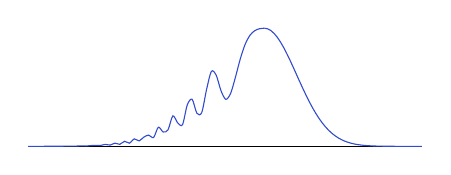
\begin{tikzpicture}[yscale=1.5]
      \draw (-3, 0) -- (2, 0);
      \draw [domain=0:2,samples=50, mblue] plot (\x, {exp(-3 * \x * \x)});
      \draw [domain=-3:0,samples=50, mblue] plot [smooth] (\x, {exp(-\x * \x) *(1 - 0.5 * sin(400*\x*\x) * sin(400*\x*\x))});
    \end{tikzpicture}
  \end{center}
  We write this as a superposition of plane wave modes. As we let time pass, different plane wave modes travel at different speeds, so this becomes a huge mess!

  Intuitively, this tells us that the third order derivative $\partial^3_x$ is what gives us dispersion.
\end{eg}

\begin{eg}
  Consider the non-linear PDE
  \[
    u_t - 6 uu_x = 0.
  \]
  This looks almost intractable, as non-linear PDE's are scary, and we don't know what to do. However, it turns out that we can solve this for any initial data $u(x, 0) = f(x)$ via the method of characteristics. The solution we get is
  \[
    u(x, t) = f(\xi),
  \]
  where $\xi$ is given implicitly by
  \[
    \xi = x - 6t f(\xi)
  \]
  We can show that $u_x$ becomes, in general, infinite in finite time. Indeed, we have
  \[
    u_x = f'(\xi) \frac{\partial \xi}{\partial x}.
  \]
  We differentiate the formula for $\xi$ to obtain
  \[
    \frac{\partial \xi}{\partial x} = 1 - 6tf'(\xi) \frac{\partial \xi}{\partial x}
  \]
  We can then check that this would indeed go to infinity in finite time, so eventually we have a straight slope. \emph{After} that, it becomes a multi-valued function! So the solution might evolve like this:

  \begin{own}
    I need some pictures.
  \end{own}
  % insert picture

  This is known as \term{wave-breaking}.

  Intuitively, we think that $-6uu_x$ corresponds to wave breaking.
\end{eg}

What happens if we combine both of these effects?
\begin{defi}[KdV equation]\index{KdV equation}
  The \emph{KdV equation} is given by
  \[
    u_t + u_{xx} - 6 u u_x = 0.
  \]
\end{defi}
It turns out that this has a perfect balance between dispersion and non-linearity. This admits very special solutions known as \term{solitons}. For example, a $1$-solution solution is
\[
  u(x, t) = -2x^2 \sech^2 (x(x - 4xt)).
\]
The solutions tries to both topple over and disperse, and it turns out they actually move like normal. Note that the speed depends on the amplitude. So we can try to put a big one before a small one, and see what happens. It turns out they just walk pass through each other, and it seems like it is just a superposition. But the KdV solution is not linear! It does not follow the superposition principle!

These solitons are a bit like particles, and they have very little interactions with other things. They are very stable structures in the system, and that is why physicists like them a lot. We will later see that the system is in fact integrable, and we will find general $n$-soliton solutions.

\subsection{Sine-Gordon equation}

\begin{defi}[Sine-Gordon equation]\index{sine-Gordon equation}
  The \emph{sine-Gordon equation} is given by
  \[
    u_{tt} - u_{xx} + \sin u = 0.
  \]
\end{defi}
This is known as the sine-Gordon equation, because there is a famous equation in physics known as the \emph{Klein-Gordon equation}, given by
\[
  u_{tt} - u_{xx} + u = 0.
\]
Since we have a sine instead of a $u$, we call it a sine-Gordon equation!

Now let's try to motivate the equation.

Consider pendulums of length $\ell$, masses $m$ on a very long spring
\begin{center}
  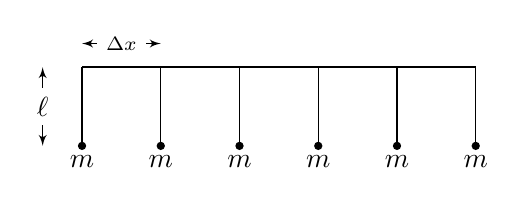
\begin{tikzpicture}
    \draw [thick] (0, 0) -- (5, 0);
    \foreach \x in {0,1,2,3,4,5} {
      \draw (\x, 0) -- (\x, -1) node [circ] {} node [below] {$m$};
    }
    \draw [latex'-latex'] (0, 0.3) -- (1, 0.3) node [pos=0.5, fill=white] {\scriptsize$\Delta x$};

    \draw [latex'-latex'] (-0.5, 0) -- (-0.5, -1) node [pos=0.5, fill=white] {$\ell$};
  \end{tikzpicture}
\end{center}
We set the pendulum in motion, and let the angle of the $i$th pendulum be $\theta_i(t) = \theta(i \Delta x, t)$ for $i \in \Z$. The gravity gives a torque of
\[
  -m\ell g \sin \theta_i.
\]
We would also expect a torque from neighbouring pendulums of magnitude, say,
\[
  \frac{K(\theta_{i + 1} - \theta_i)}{\Delta x},\quad \frac{K(\theta_{i - 1} - \theta_i)}{\Delta x}.
\]
(it doesn't really matter. We don't really care about pendulums)

By Newton's laws, we get
\[
  m\ell^2 \frac{\d^2 \theta_i}{\d t^2} = -mg \ell \sin \theta_i + \frac{K(\theta_{i + 1} - 2 \theta_i + \theta_{i - 1})}{\Delta x}.
\]
We divide everything by $\Delta x$, and take the limit as $\Delta x \to 0$, with $M = \frac{m}{\Delta x}$ held constant. We then end up with
\[
  M \ell^2 \frac{\partial^2 \theta}{\partial t^2} = - Mg\ell \sin \theta + K \frac{\partial^2 \theta}{\partial x^2}.
\]
Making some simple coordinate scaling, this becomes
\[
  u_{tt} - u_{xx} + \sin u = 0.
\]
There is also another motivation for this from differential geometry. It turns out solutions to the sine-Gordon equation correspond to pseudospherical surfaces in $\R^3$, namely the surfaces that have constant zero curvature.

This also admits solitons solutions
\[
  u(x, t) = 4 \tan^{-1} \left(\exp\left(\frac{x - vt}{\sqrt{1 - v^2}}\right)\right).
\]
We can check that this is indeed a solution for this non-linear PDE.

It turns out these solutions look like
\begin{center}
  \begin{tikzpicture}[xscale=0.5]
    \draw [->] (-8, 0) -- (8, 0);
    \draw [->] (-4, -0.5) -- (-4, 3);
    \draw [thick, blue] (0, 0) -- (0.01, 0);
    \draw [domain=-8:8, thick, blue] plot [smooth] (\x, {atan (exp (\x)) / 45});

    \draw [dashed] (-8, 2) -- +(16, 0);
    \node [anchor = north east] at (-4, 2) {$2\pi$};
% \draw [domain=0.01:0.99, thick, blue] plot [smooth] (\x, {2 * (exp(- 1 / (\x * \x)))/((exp(- 1 / (\x * \x))) + (exp(- 1 / ((1 - \x) * (1 - \x)))))});
  \end{tikzpicture} % max is 2pi
\end{center}
Now remember that $\theta$ was an angle. So $2\pi$ is just the same as $0$! If we think of $u$ as living in $S^1$, then this satisfies the boundary condition $u \to 0$ as $x \to \pm \infty$, and we also know that no matter how this evolves, we will never get rid of this ``loop''. So the soliton is stable.


\end{document}
